\documentclass[a4paper,10pt]{article}
\usepackage[T1]{fontenc}
\usepackage[utf8]{inputenc}
\usepackage[italian]{babel}
\usepackage[top=2.25cm, bottom=2.25cm, left=2.25cm, right=2.25cm]{geometry}
\usepackage{graphicx}
\graphicspath{{/home/egg/uni/root/RootSimulation/build/analysis/}}
\usepackage{subfig}
\usepackage{amsmath}
\usepackage{booktabs}
\usepackage{multirow}
\usepackage{caption}
\captionsetup[table*]{position=top}
\captionsetup[figure*]{position=bottom}
\usepackage{dblfloatfix}
\usepackage[hidelinks]{hyperref}
\usepackage{lipsum}

\usepackage[dvipsnames]{xcolor}
\definecolor{veryLightGrey}{rgb}{0.9629411,0.9629411,0.9629411}
\usepackage{listings}
\renewcommand{\lstlistingname}{Listato}
\renewcommand{\lstlistlistingname}{Indice dei listati}

\lstset{
inputpath=/home/egg/uni/root/RootSimulation/,
language=c++,
basicstyle=\ttfamily\footnotesize,
commentstyle=\fontseries{lc}\selectfont\itshape\color{OliveGreen},
numbers=left,
numberstyle=\ttfamily\footnotesize,
stepnumber=1,
numbersep=5pt,
backgroundcolor=\color{veryLightGrey},
showspaces=false,
showstringspaces=false,
showtabs=false,
frame=tb,
tabsize=4,
captionpos=t,
breaklines=false,
%commentstyle=\color{OliveGreen},
stringstyle=\color{BrickRed},
keywordstyle=\color{RoyalBlue}
}

\title{Relazione ROOT}
\author{Nicolò Montalti}
\date{\today}

\begin{document}
\maketitle
\section{Introduzione}
Il programma si divide in due parti: una di generazione e una di analisi. Nella prima vengono generati $10^5$ gruppi di 100 particelle ciascuno secondo proporzioni predefinite. Le particelle possono essere pioni, kaoni o protoni, tutte di carica positiva o negativa. In aggiunta è possibile produrre kaoni di risonanza, dal cui decadimento si ottengono un pione e un kaone di carica opposta.

Durante la fase di analisi si verifica che la generazione sia coerente con i parametri impostati. Si controllano l'abbondanza dei vari tipi di particelle, la distribuzione del modulo dell'impulso e la sua direzione. Si cerca inoltre di risalire alla massa e alla vita media delle $K^*$ decadute. Ciò avviene analizzando gli istogrammi della massa invariante calcolata tra vari gruppi di particelle. La massa invariante tra i prodotti delle $K^*$ decadute si distribuisce infatti secondo una distribuzione gaussiana la cui media è legata alla massa delle $K^*$ e la deviazione standard all'inverso della vita media.

\section{Struttura del codice}
Alla base del programma ci sono tre classi: ParticleType, ResonanceType e Particle. La classe ParticleType (list.~\ref{ParticleType.hpp}-\ref{ParticleType.cpp}) contiene la massa, la carica e il nome di ogni tipo di particella. Dispone inoltre dei rispettivi getters e di un metodo Print che permette di stampare a schermo ogni informazione. La classe ResonanceType (list.~\ref{ResonanceType.hpp}-\ref{ResonanceType.cpp}) eredita da ParticleType e aggiunge la larghezza di risonanza con il rispettivo getter. Sovrascrive inoltre il metodo Print, in modo da stampare anche quest'ultimo attributo. Si è scelto di fare ereditare ResonanceType da ParticleType perché le due classi sono in una relazione di tipo "is-a". Ogni particella di risonanza è anche una particella in senso generale e ne possiede tutti gli attributi (nome, massa e carica).

La classe Particle (list.~\ref{Particle.hpp}-\ref{Particle.cpp}) aggiunge le proprietà cinematiche tipiche di una particella fisica, cioè le tre componenti della quantità di moto. Per integrare le informazioni sulla specie si è scelto di non fare ereditare Particle da ParticleType. Se si fosse sfruttata l'ereditarietà, per ogni istanza di Particle sarebbero stati salvati in memoria nome, massa e carica, sprecando risorse. Si è preferito utilizzare l'aggregazione e includere nella classe Particle un array statico di puntatori ParticleType e un indice intero. L'array è riempito tramite il metodo statico AddParticleType all'inizio del programma. Ogni istanza di Particle viene inizializzata con un indice che indica il tipo di particella. Oltre ai canonici getters e setters, Particle dispone di un metodo Decay2Body che permette ai $K^*$ di decadere in un pione e in un kaone di carica opposta.

\section{Generazione}
La generazione avviene nel file main.cpp (list.~\ref{main.cpp}). Inizialmente vengono generati $10^5$ eventi di 100 particelle ciascuno. Ad ogni particella viene assegnata una specie casuale attraverso un blocco if-else if-else secondo le proporzioni definite in tab.~\ref{tab:proporzioni}. La quantità di moto è stabilita estraendone il modulo da una distribuzione esponenziale di media 1 GeV. Gli angoli azimutali e polari si ricavano invece da due distribuzioni uniformi definite sugli intervalli $[0,\pi]$ e $[0,2\pi]$. Le particelle $K^*$ vengono fatte decadere in un $\pi^+$ e un $K^-$ o in $\pi^-$ e un $K^+$ con pari probabilità. Tutte le estrazioni si basano sulle distribuzioni standard di ROOT, richiamate attraverso il puntatore globale gRandom.

\begin{table*}
  %  \caption{Caratteristiche e abbondanza delle particelle generabili e analizzabili dal programma}
  %  \centering
  %  \subfloat[Particelle generabili e rispettive proporzioni]{
  \caption{Proporzioni e caratteristiche delle particelle generate}
  \label{tab:proporzioni}
  \centering
  \begin{tabular}{cccc}
    \toprule
    Particella               & Carica (e) & Simbolo & Percentuale \\
    \midrule
    \multirow{2}{*}{Pione}   & +1         & $\pi^+$ & 40\%        \\
                             & -1         & $\pi^-$ & 40\%        \\
    \midrule
    \multirow{3}{*}{Kaone}   & +1         & $K^+$   & 5\%         \\
                             & -1         & $K^-$   & 5\%         \\
                             & 0          & $K^*$   & 1\%         \\
    \midrule
    \multirow{2}{*}{Protone} & +1         & $p^+$   & 4.5\%       \\
                             & -1         & $p^-$   & 4.5\%       \\
    \bottomrule
  \end{tabular}
\end{table*}

Durante la generazione vengono riempiti una serie di istogrammi. Vengono salvati i tipi di particella generati, il modulo e la direzione dell'impulso, l'energia e la massa invariante. In particolare per la massa invariante vengono creati cinque istogrammi. Nel primo la massa invariante viene calcolata tra tutte le particelle di ogni evento; in altri due solo tra le particelle di carica uguale e di carica opposta; negli ultimi solo tra un pione e un kaone di carica uguale e di carica opposta. Tutti gli istogrammi vengono poi salvati in un file ROOT per essere analizzati successivamente.

\section{Analisi}
L'analisi è codificata nel file analysis.cpp (list.~\ref{analysis.cpp}). Come si può osservare nella tab.~\ref{tab:abbondanza} e nel primo istogramma in fig.~\ref{fig:Generation}, l'abbondanza delle varie specie è compatibile con i valori attesi. Il modulo dell'impulso si distribuisce secondo una distribuzione esponenziale di media compatibile con il valore atteso 1 GeV e con un $\chi^2$ accettabile. Allo stesso modo gli angoli azimutali e polari dell'impulso sono compatibili con una distribuzione uniforme definita sui rispettivi domini.

Per risalire alle caratteristiche delle $K^*$ decadute si è sfruttato il fatto che ogni decadimento produca un kaone e un pione di carica opposta. L'insieme delle particelle di carica concorde contiene quindi solo particelle che non sono state originate da un decadimento, mentre quello delle particelle di carica opposta contiene le particelle originate dai decadimenti più le altre. Sottraendo il secondo dal primo si elimina gran parte del fondo delle particelle non originate dai decadimenti. Fittando l'istogramma delle masse invarianti tra questo gruppo di particelle si ottiene una gaussiana con media pari alla massa delle $K^*$ e deviazione standard pari alla larghezza di risonanza. In tab.~\ref{tab:fitgaus} è riportato l'esito del fit.

Per migliorare la precisione della misura si è riutilizzato il metodo appena descritto restringendolo ai soli pioni e kaoni, dato che i decadimenti non producono protoni. In tab.~\ref*{tab:fitgaus} sono riportati l'esito del fit e un fit gaussiano di controllo eseguito sulla massa invariante tra le coppie $\pi K$ prodotte dai decadimenti. In fig.~\ref*{fig:InvMass} sono riportati i tre istogrammi della massa invariante coi rispettivi fit.

Gli esiti di tutti e tre i metodi di calcolo restituiscono $\chi^2$ accettabili e sono compatibili con i valori attesi di media (0.89166~GeV/c$^2$) e deviazione standard (0.050~GeV/c$^2$).
% , ad eccezione della $\sigma$ della massa invariante calcolata tra i prodotti dei decadimenti delle $K^*$, per cui la discrepanza è significativa ($p = 0.037$). Anche ripetendo la generazione non si è riuscito ad eliminare la discrepanza.
È infine rilevante notare come restringendo il calcolo ai soli pioni e kaoni l'errore si riduca sensibilmente.

\begin{table}
  \caption{Abbondanza attesa e osservata delle particelle generate divise per tipo}
  \label{tab:abbondanza}
  \centering
  \begin{tabular}{cccc}
    \toprule
    Specie  & Occorrenze osservate $(10^5)$ & Occorrenze attese $(10^5)$ \\
    \midrule
    $\pi^+$ & 40.01 $\pm$ 0.02              & 40                         \\
    $\pi^-$ & 40.00 $\pm$ 0.02              & 40                         \\
    $K^+$   & 4.995 $\pm$ 0.007             & 5.0                        \\
    $K^-$   & 4.996 $\pm$ 0.007             & 5.0                        \\
    $p^+$   & 4.493 $\pm$ 0.007             & 4.5                        \\
    $p^-$   & 4.495 $\pm$ 0.007             & 4.5                        \\
    $K^*$   & 1.007 $\pm$ 0.003             & 1.0                        \\
    \bottomrule
  \end{tabular}
\end{table}


\begin{table}[p]
  \caption{Fit del modulo e degli angoli azimutali e polari dell'impulso delle particelle generate}
  \label{tab:fit}
  \centering
  \begin{tabular}{cccccc}
    \toprule
    Variabile        & Distribuzione & Parametro del fit                     & $\chi^2$ & DOF & $\chi^2$/DOF \\
    \midrule
    Modulo           & expo          & (1.0001 $\pm$ 0.0003) GeV             & 23.79    & 18  & 1.32         \\
    \midrule
    Angolo azimutale & pol0          & $(10000 \pm 3) \cdot 10^2$ rad$^{-1}$ & 9.50     & 9   & 1.06         \\
    Angolo polare    & pol0          & $(10000 \pm 3) \cdot 10^2$ rad$^{-1}$ & 14.03    & 9   & 1.56         \\
    \bottomrule
  \end{tabular}
\end{table}

\begin{figure*}[p]
  \centering
  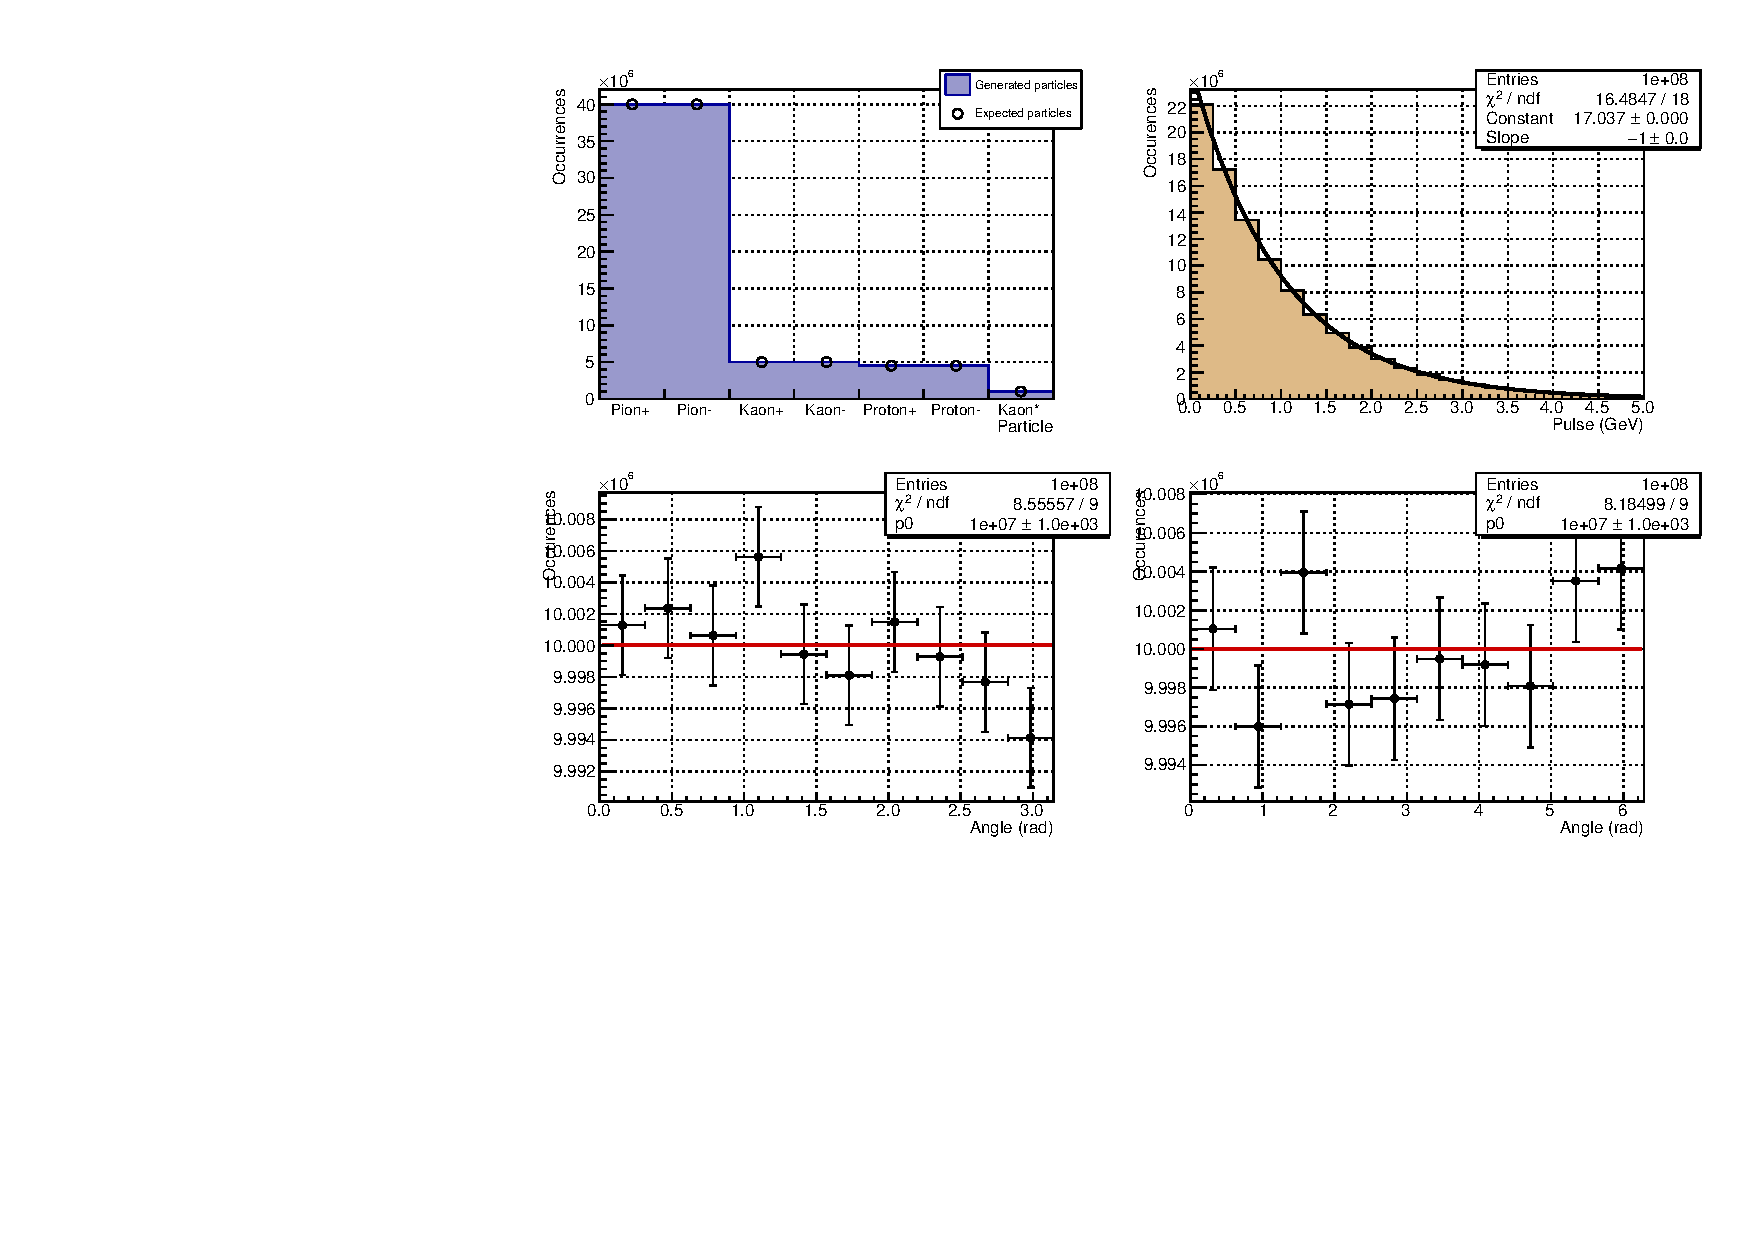
\includegraphics[width=\linewidth]{Generation.pdf}
  \caption{Istogrammi delle particelle generate e attese divise per specie (in alto a sx), del modulo dell'impulso con fit esponenziale (in alto a dx) e degli angoli azimutali e polari con fit pol0 (rispettivamente in basso a sx e a dx)}
  \label{fig:Generation}
\end{figure*}

\begin{table*}
  \caption{Fit degli istogrammi della massa invariante calcolata tra varie combinazioni di particelle}
  \label{tab:fitgaus}
  \centering
  \begin{tabular}{p{4.5cm}cccc}
    \toprule
    Distribuzione gaussiana                                                                                        & Media (Gev/c$^2$)     & Sigma (GeV/c$^2$)     & Ampiezza ($10^4$) & $\chi^2$/DOF \\
    \midrule
    Massa invariante ottenuta dalla differenza delle combinazioni di particelle di carica discorde e concorde      & 0.888 $\pm$ 0.005     & 0.054 $\pm$ 0.006     & 3.8 $\pm$ 0.3     & 0.43         \\
    \midrule
    Massa invariante ottenuta da differenza delle combinazioni di particelle $\pi K$ di carica discorde e concorde & 0.892 $\pm$ 0.002     & 0.049 $\pm$ 0.002     & 1.99 $\pm$ 0.07   & 1.36         \\
    \midrule
    Massa invariante ottenuta dalle particelle generate dai decadimenti delle $K^*$                                & 0.89146 $\pm$ 0.00016 & 0.05015 $\pm$ 0.00011 & 1.335 $\pm$ 0.005 & 1.57         \\
    \bottomrule
  \end{tabular}
\end{table*}

\begin{figure*}[t]
  \centering
  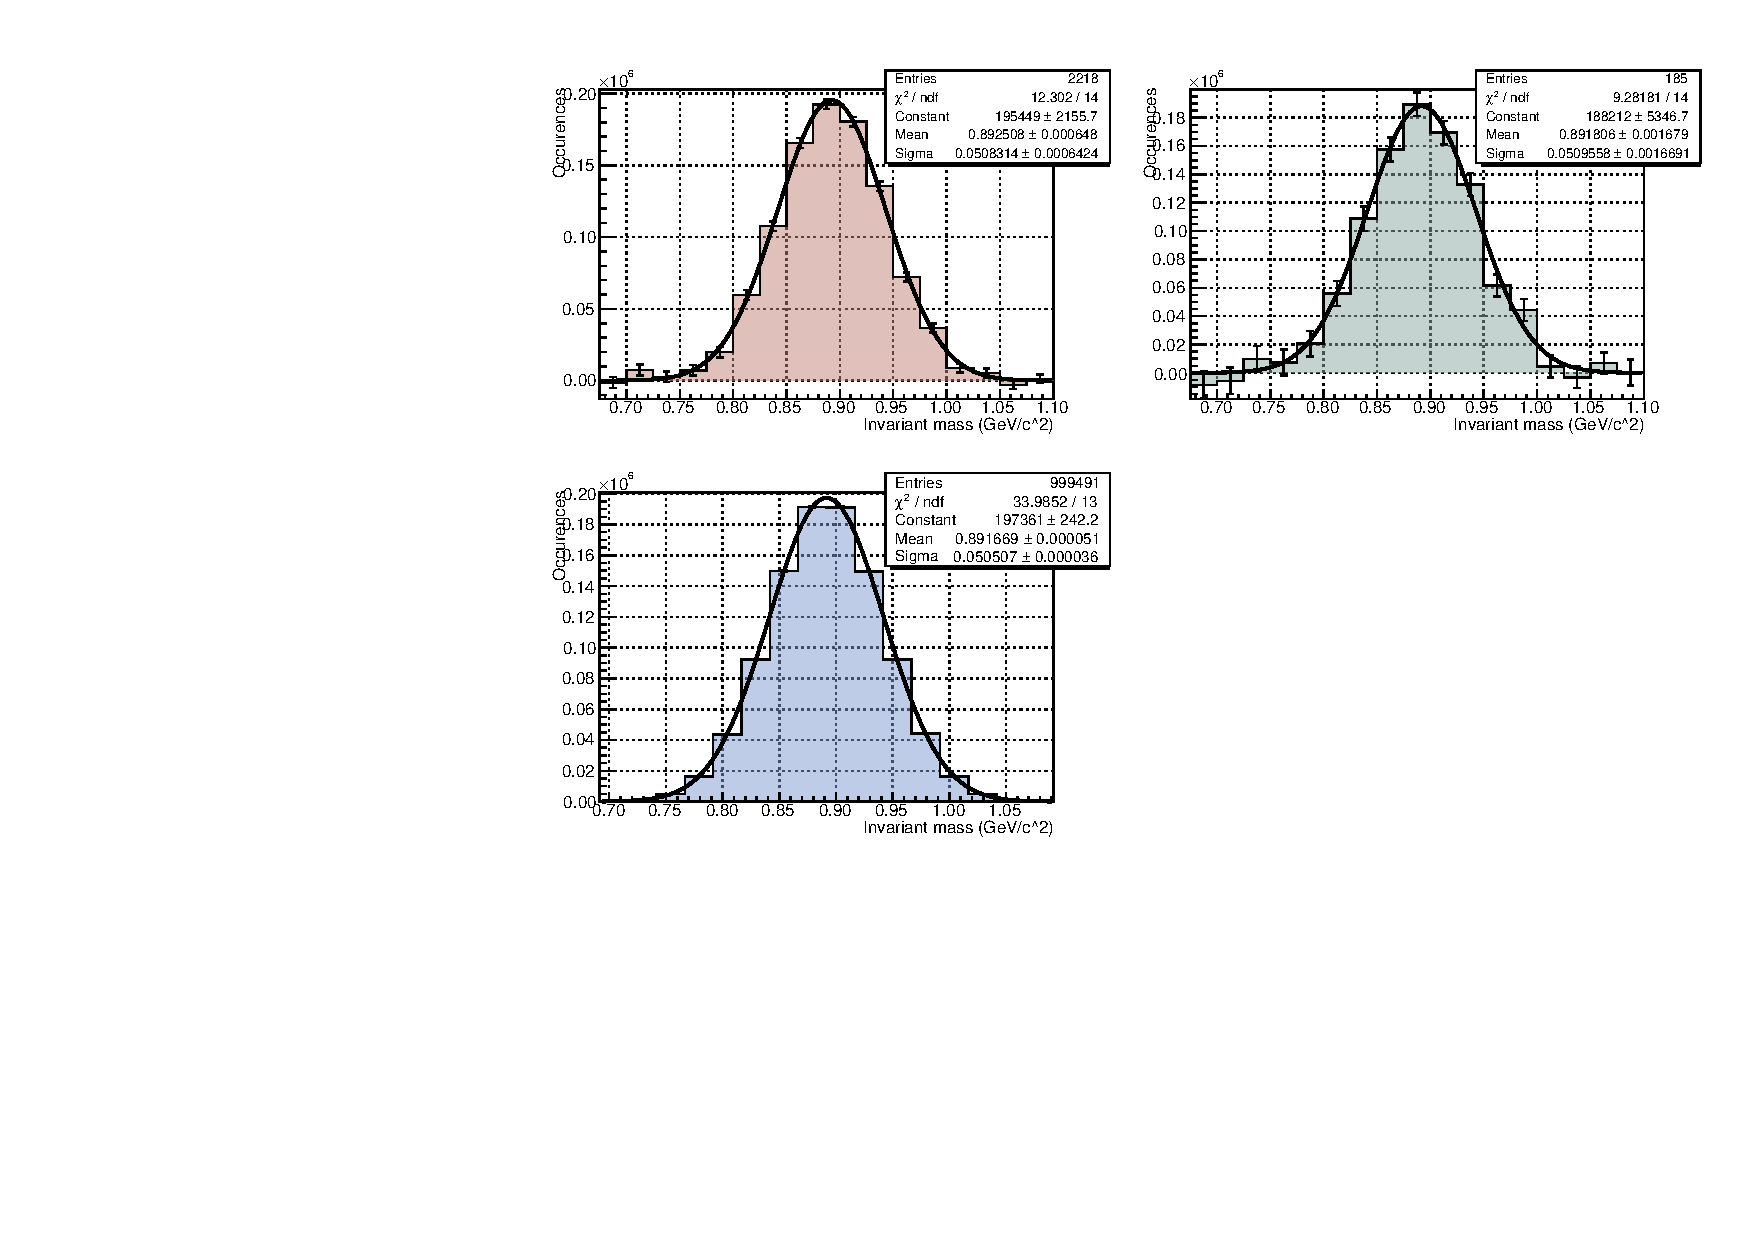
\includegraphics[width=0.95\linewidth]{InvMass.pdf}
  \caption{Istogrammi della massa invariante ottenuta dalla differenza di combinazioni di particelle di carica uguale ed opposta (in alto a sx), dalla differenza delle combinazioni $\pi K$ di carica uguale ed opposta (in alto a dx) e dalle coppie $\pi K$ generate dai decadimenti delle $K^*$ (in basso a sx)}
  \label{fig:InvMass}
\end{figure*}

\newpage
\lstlistoflistings
\lstinputlisting[caption=particleType.hpp, label=ParticleType.hpp]{generation/ParticleType.hpp}
\lstinputlisting[caption=particleType.cpp, label=ParticleType.cpp]{generation/ParticleType.cpp}
\lstinputlisting[caption=resonanceType.hpp, label=ResonanceType.hpp]{generation/ResonanceType.hpp}
\lstinputlisting[caption=resonanceType.cpp, label=ResonanceType.cpp]{generation/ResonanceType.cpp}
\lstinputlisting[caption=particle.hpp, label=Particle.hpp]{generation/Particle.hpp}
\lstinputlisting[caption=particle.cpp, label=Particle.cpp]{generation/Particle.cpp}
\lstinputlisting[caption=main.cpp, label=main.cpp]{generation/main.cpp}
\lstinputlisting[caption=analysis.cpp, label=analysis.cpp]{analysis/analysis.cpp}
\lstinputlisting[caption=myStyle.hpp, label=myStyle.hpp]{analysis/myStyle.hpp}

\end{document}
